\section{Mathematical view on network training}
\par{}
Consider an example network shown in \cref{example_network}. Here, the input
data \(x\) is fed to a fully connected network that estimates the output
data \(\hat{y}\), which then compared with the expected output data \(y\) through
loss function.  \\

\begin{figure}
    \center
    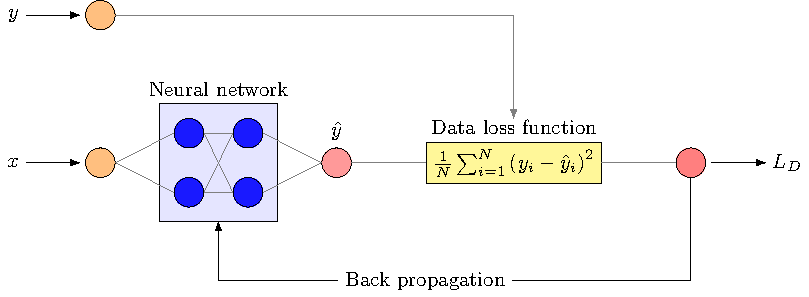
\includegraphics[scale=1]{supportingFiles/01_schematics/01_NN_example/NN_example.pdf}
    \caption{Example network}
    \label{example_network}
\end{figure}

\par{}
Weights and biases of the example network were then optimized with loss as
objective function, minimizing it to match the expected output values through
an algorithm called back propagation. The main reference for this back
propagation equations for a fully connected network is
\cite{backpropagation_reference}. \\

\par{}
Mathematically, a single layer \(l\) is represented as given below.
\begin{align*}
    \bm{x}^{[l]} = \sigma\left( \bm{z}^{[l]}\right)
\end{align*}

where,
\begin{align*}
    \bm{z}^{[l]} = \bm{W}^{[l]}\cdot\bm{x}^{[l-1]} + \bm{b}^{[l]}
\end{align*}

Here, \(\bm{W}^{[l]}\) is the weight matrix and \(\bm{b}^{[l]}\) is the bias
vector of layer \(l\).  \(\bm{x}^{[l-1]}\) is the activated output of the
previous layer \(l-1\), and \(\sigma\) is the activation function. Let, \(L\)
be the loss function evaluated at the end of last layer. Then, the gradient of
loss function with respect to the unactivated output of last layer\(z^{[l]}\)
is given as below.

\begin{align}
    \left.\frac{\partial L}{\partial \bm{z}^{[l-1]}} = \left[\bm{W}^{[l]} \right]^T \cdot \frac{\partial L}{\partial \bm{z}^{[l]}} * \frac{\partial \sigma}{\partial \bm{z}}\right\vert_{[l-1]} \label{error_eqn}
\end{align}

\Cref{error_eqn} is called as the error of a layer. The error is back
propagated from layer \(l\) to the previous layer \(l-1\) by the above
equation.  Here, \(*\) is the element-wise multiplication. To begin this back
propagation, we need the above error derivative \(\partial L/\partial z\) for
the last layer in the network. \\

\par{}
The computation of error for the last layer will involve the differentiation
of loss function \(L\) with respect to the estimated output \(\hat{y}\). Let
the last layer be described as given below.
\begin{align*}
    \bm{\hat{y}} = \sigma\left(\bm{z}\right)
\end{align*}

And, let the loss function be the classical mean squared error as given below.
\begin{align*}
    L = \frac{1}{N}\sum_{i=1}^{N} \left(\hat{y}_i - y_i\right)^2
\end{align*}

Then, the error for the last layer is calculated as shown below.
\begin{align*}
    \left.\frac{\partial L}{\partial \bm{z}}\right\vert_{[l]} = \frac{\partial L}{\partial \bm{\hat{y}}} \cdot \frac{\partial \bm{\hat{y}}}{\partial \bm{z}} = \frac{\partial L}{\partial \bm{\hat{y}}} \cdot \frac{\partial \sigma}{\partial \bm{z}} = \left(\frac{2}{N}\sum_{i=1}^{N}\left(\hat{y}_i - y_i\right)\right) \left.\frac{\partial \sigma}{\partial \bm{z}}\right\vert_{[l]}
\end{align*}

Hence, the above equation completes the error computation for all the layers, next
we have to compute the derivatives of loss with respect to weights and
biases of all the layers using these error vectors. The gradients of loss with
respect to weights and biases are computed using the error vector for each layer
as shown below.
\begin{align}
    \frac{\partial L}{\partial \bm{W}^{[l]}} &= \frac{\partial L}{\partial \bm{z}^{[l]}} \cdot \left[\bm{x}^{[l-1]}\right]^T \label{weight_eqn} \\
    \frac{\partial L}{\partial \bm{b}^{[l]}} &= \frac{\partial L}{\partial \bm{z}^{[l]}} \label{bias_eqn}
\end{align}

So, with the above gradient equations \cref{error_eqn,weight_eqn,bias_eqn}, the
weights and biases of all the layers can be computed and optimized with aim of
minimizing the loss function. An example problem with data-driven network is
given below that was solved with the neural network built using above
equations.
